\section{Multiband Mesh Architecture and Model}
\label{sec:architecture}

% Organization of the Sec
In this section, we first introduce the 
~\emph{Multiband Mesh Network Architecture}
with white space band propagation, connectivity and interference characteristics.
Then we analysis the architecture and formulate the architecture into a graph model with hypothesis.

\subsection{Multiband Mesh Network Architecture}
\label{subsec:architecture}
Generally ~\emph{Wireless Mesh Network} is been described as two-tiers:
Consisting of an access layer for clients to mesh nodes, and a backhual layer for interconnection from mesh nodes to gateway nodes with wired Internet connection ~\cite{akyildiz2005wireless}. 
Nodes in backhual layer are static.
Our work focus on ~\emph{Wireless Mesh Network} with ~\emph{White Space Frequency} in backhual layer. 
The clients devices in industrial, scientific and medical (ISM) band, such as iPhone, laptops, access to mesh node with independent channel of ISM band from backhual layer. 

% Explain multiband vs multichannel
A lot of efforts have been put on ~\emph{Multichannel Multi-radio Mesh Network} architecture focusing on ~\emph{Gateway Placement, Channel Assignment, Multihop Routing} problems ~\cite{si2010overview}.
~\emph{Multichannel} is a word mention different frequency channels with small gap, for instance the orthogonal WLAN channels in 2.4GHz from 2.412GHz to 2.484GHz with 22MHz gap.
We refer ~\emph{Multiband} with a combination of different frequency of large gap, such as a set 2.4GHz and 900MHz whose propagation characteristics are different.

% Explain propagation, factors of the environment and so on
Wireless propagation is the behavior of the signal loss characteristics when they are transmitting from one point to another.
The factors rule radio propagation are complex and diverse, and in most propagation models there are three basic propagation mechanisms: reflection, diffraction, and scattering ~\cite{andersen1995propagation}.
Wireless propagation could be affected by the daily changes of environment, weather, and atmosphere changes due to cosmos activities. 
In multiband mesh backhual layer, the nodes are usually installed on the top of buildings or towers. That makes a line of sight propagation model is a reasonable hypotheses for multiband mesh.
% propagation fomular, explain the band influence
In a popular propagation model \emph{Friis Model}, the received signal power of a node is represented as: 
\begin{equation}
\label{eq:friis}
P_r=P_t+G_t+G_r+20log_{10}(\frac{\lambda}{4\pi R})
\end{equation}

Path-loss exponent \emph{$\alpha$} is used to describe the environment factors, typically in outdoor environments range from 2 to 5.\cite{camp2006measurement}. 
The received signal could be different only related to the wavelength $\lambda$ represents band. 
The propagation difference makes the performance of radios in different bands vary with the same configuration in the same location. With the same received signal threshold, lower frequency band could have a larger propagation range $R$.

In multiband scenario, both wired ~\emph{Gateway Nodes} and ~\emph{Mesh Nodes} are equipped with multiple radios working in different frequency band, including ISM bands and white space bands. The radios could work simultaneously bringing more capacity to the network which is a evolution of ~\emph{Multi-channel Multi-Radio Mesh Network} with radios working in the same band in different channels.

\begin{figure}                                                                                                                     
%\vspace{-0.0in}
\centering
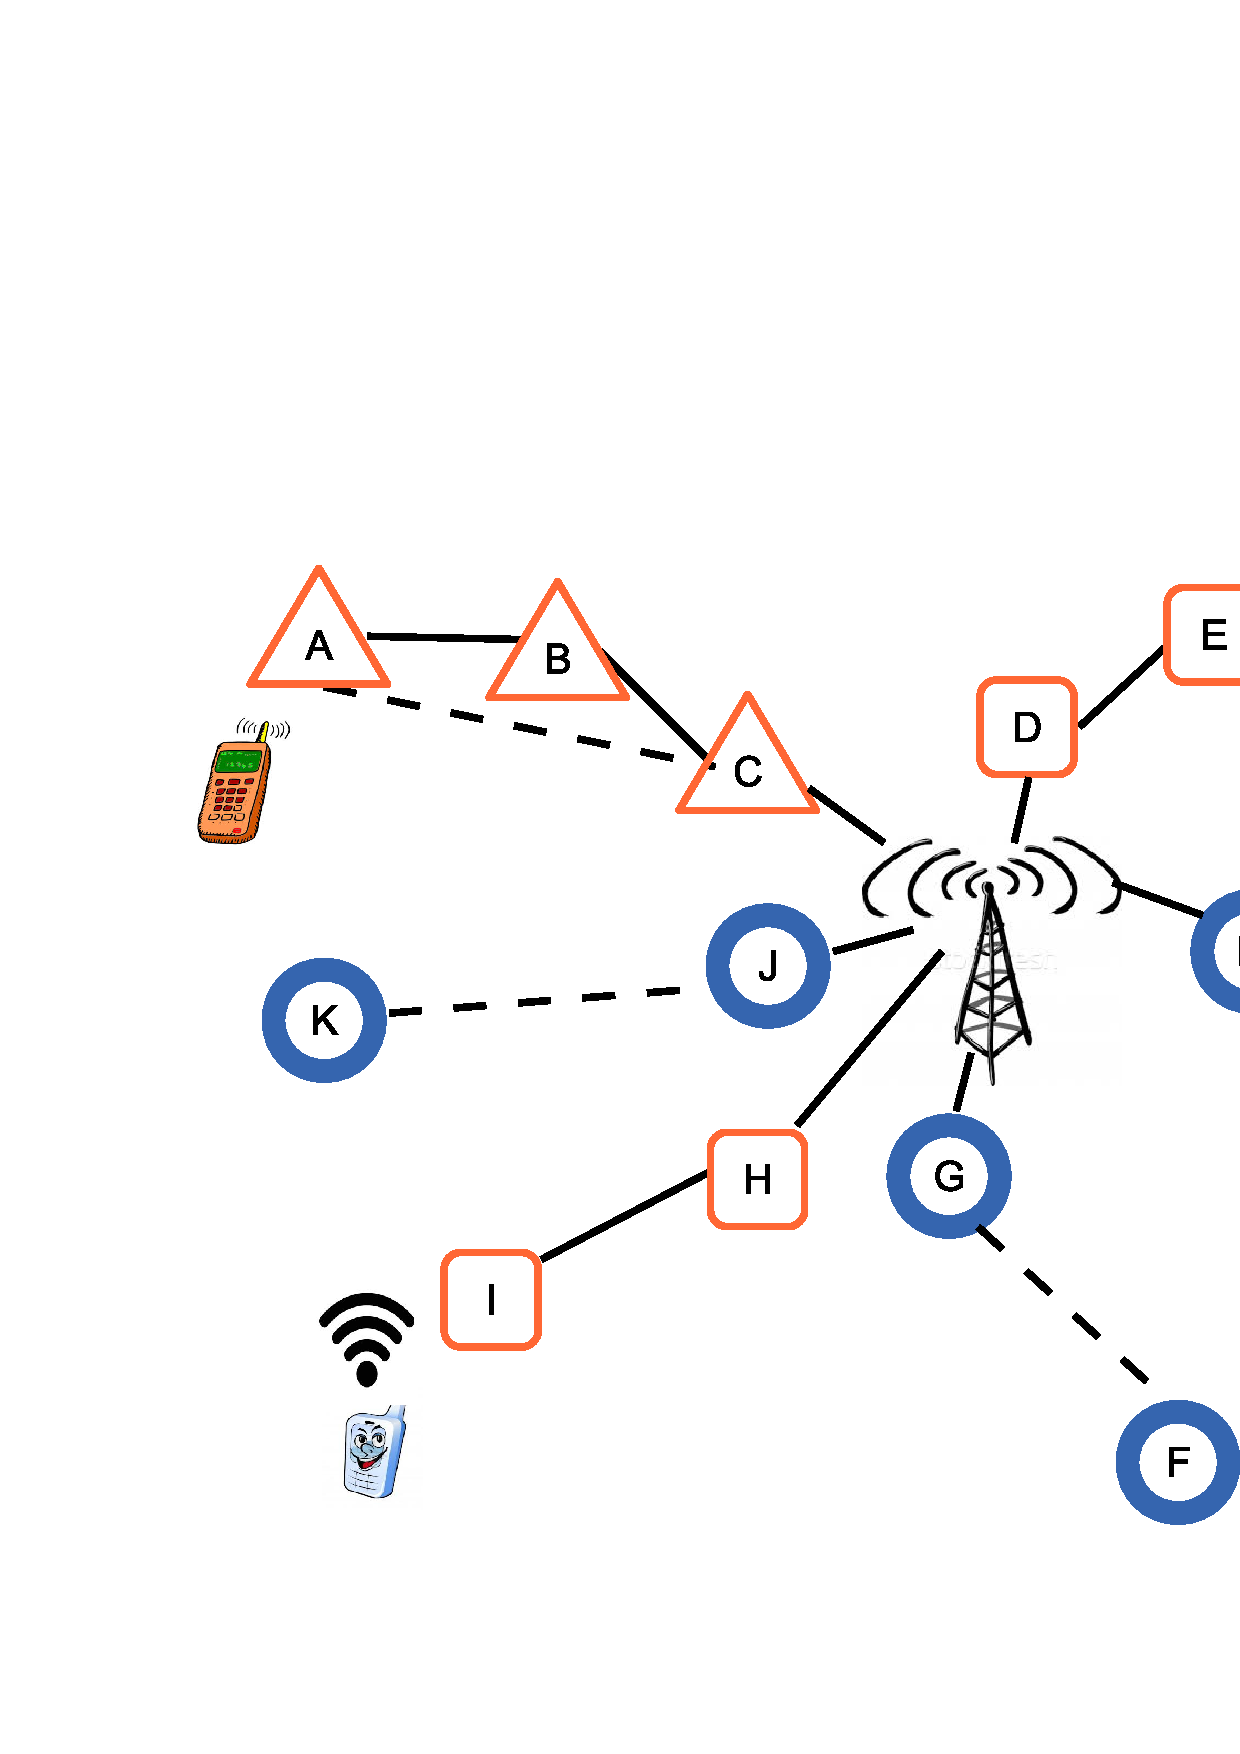
\includegraphics[width=74mm]{figures/interferencerange}
\vspace{-0.1in}
\caption{Multiband Communication and Interference Range}
\label{fig:interferencerange}
%\vspace{-0.0in}
\end{figure}


% Make multiband networks interesting 
The broadcast nature of the wireless medium makes it generate multiple access interference.
Employing ~\emph{White Space Band} in lower frequency brings advantages for mesh network, 1) more orthogonal bandwidth make the contention in the network lower,
 2) the propagation difference brings flexible topology by reduce connection hop counts in the network.
However, at the same time, ~\emph{White Space Band} also increase the interference range in the network making more interference in the same band. Both goods and bad are embedded in ~\emph{White Space Band} for mesh network.
In \ref{fig:interferencerange}, node ~\emph{N1} could connect to node ~\emph{N3} relay on node ~\emph{N2} in higher frequency band or through lower frequency band directly.
If under higher frequency band, link between node ~\emph{N4} and node ~\emph{N5} could reuse the higher frequency because they are out of the interference range of this high frequency band; however, if \emph{N1} and ~\emph{N3} use lower frequency band with less hop count, then ~\emph{N4} and ~\emph{N5} could not reuse the lower frequency due to the larger interference range.
To balance the larger communication range and larger interference range of white space band is a key issue in ~\emph{Multiband Mesh Network Channel Assignment}.

\subsection{Model and Problem Formulation}
\label{subsec:problem}

% Assumptions of the network
~\emph{Channel Assignment} is to assign radios between nodes in mesh network creating virtual links for network communication with minimum interference.
We consider a wireless mesh network formed by a set of stationary mesh nodes and wired gateway nodes. Each node is equipped with one or more radios in different bands. To clarify the ~\emph{White Space Band} influence, we assume radios in a node works in unique non-overlapping channels of multiple band, radios in two nodes share a common channel in the same band.
All the radios work under the same transmitting power, antenna with the same gains.
To model the connectivity, we adopt classical ~\emph{Protocol Model} from Gupta ~\cite{gupta2000capacity}. If the received signal is above the threshold, the link would have a communication capacity, otherwise, the link could not exist.
For the interference, when the received signal is above the interference threshold, there will be contention exist; otherwise, the signal will not influence other links.

The ~\emph{Gateway Nodes} and ~\emph{Mesh Nodes} locations have been known as input. In a network, ~\emph{Channel Assignment} naturally binds with a routing protocol for application, but have different target. We bind our model with a ~\emph{Shortest Path Routing} protocol for ~\emph{Channel Assignment} application and evaluation.

From the input nodes location, transmitting power, antenna gains, communication and interference threshold, and bind with ~\emph{Friis Model}, we can get ~\emph{Communication Range} and ~\emph{Interference Range} of each node in different band. 
We model the connectivity between mesh nodes by an undirected graph ~\emph{Connectivity Graph}, $C=(V,L,B)$, $V$ denotes the set of nodes, $L$ denotes the set of links, $B$ denotes the set of frequency bands. A pair of nodes have a link with capacity $C_l$ in $L$ of band $b$ in $B$, if they are physically located within each others communication range of a band. 

This model associates an interference range which is larger than the communication range for each node, defining the range up to which a transmitter can interference with the reception of a link. We extend the ~\emph{Conflict Graph} from Jain's work with a flexible approach for interference, $CG=(L_{i,j},I_{Set},B)$. $L_{i,j}$ is the active link, $I_{Set}$ includes all the links are physically inside the interference range, 

Our model is similar to ~\emph{Multichannel Model} in previous works ~\cite{tang2005interference,yuan2006cross,si2010overview}. However, in ~\emph{Multichannel Model}, the ~\emph{Communication Range} and ~\emph{Interference Range} in different channels are the same. The ~\emph{Multichannel Model} is unnecessary to consider the variation of range due to band propagation.
~\emph{Multiband Channel Assignment} work toward the same target as ~\emph{Multichannel Channel Assignment} to provide richer connectivity with minimum interference with the influence on topology from the new multiband factor.

The difficulty of the problem is that we can not know the interference before we assign channel to each node. Previous works have proposed ~\emph{Coloring, Cluster, Independent Set, Mixed Linear Integer} methodology to approach the solution of ~\emph{Multichannel Channel Assignment} ~\cite{mishra2005weighted,peng2012efficient,tang2005interference}. 
However, they fails to distinguish the ~\emph{Multi-hop} and ~\emph{Conflict Graph} variation among multiple bands.
To approach the optimization channel assignment, we develop a mixed linear integer model to fit the multiband scenario. We also analyze the intra-relation between the ~\emph{Hop Counts} and ~\emph{Conflict Graph} and propose a partition and a heuristic approaching for this problem.

\subsection{Evaluation Metric}
\label{subsec:metric}
~\emph{Mesh Network} is designed to provide service for clients. The goal of a backhual network is to maximize its overall goodput within a unit time. 
This enables the network to support more end-user flows, and in turn more number of users. To evaluate the assignment, we use the idea of ~\emph{Gateway Goodput} of the network. The gateway goodput X of a network is defined as

\begin{equation}
\label{eq:goodput}
X=\sum_{g \in G, v \in V}C(g,v)
\end{equation}

In ~\cite{robinson2008adding}, Robinson proves the bottle neck of mesh network capacity is the gateway wireless connection. The gateway goodput is the traffic arrive at the gateway node and relay to the wired Internet. The goodput performance is correlated with gateway placement, channel assignment and routing. Our work focus on the channel assignment after gateway placement done, binding with shortest path routing. Jointly optimize the problem is out of the paper topic.

